%----------------------------------------------------------------------------
\chapter{Felsőszintű architektúra}
\label{sec:Architecture}
%----------------------------------------------------------------------------

\section{High level architektúra}
\label{sec:HighLevelArchitecture}

\begin{figure}[!ht]
    \centering
    \begin{tabular}{cc} % Három oszlop és két sor elrendezése
        % Első sor
        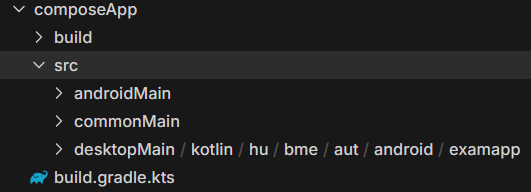
\includegraphics[width=0.35\textwidth, keepaspectratio]{figures/KmpFileStructure.png} & 
        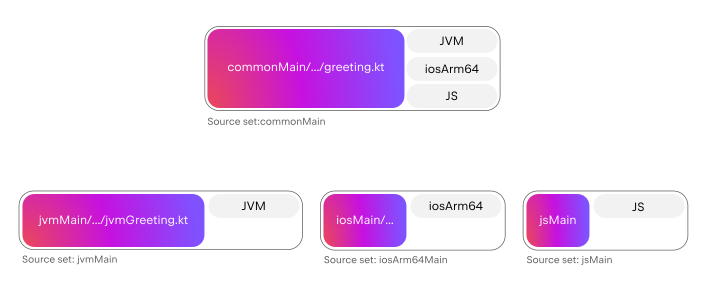
\includegraphics[width=0.65\textwidth, keepaspectratio]{figures/specific-target-diagram.png}
    \end{tabular}
    \caption{Fájl struktúrája az alkalmazásnak. Második kép: \cite{BasicProject}}
    \label{fig:FileStructure}
\end{figure}

Minden Kotlin Multiplatform projekt tartalmaz legalább 3 Main könyvtárat az src mappán belül.
Szükséges egy commonMain mappa, ami a közös kódrészleteket tartalmazza. Minél több tartalom található ebben megvalóstíva és nem külön kiszervezve annál jobb a kód újrafelhasználhatóságunk.
A többi Main mappa a platform specifikus kódrészleteket tartalmazza. Az én alaklamazásomban van egy androidMain és egy desktopMain, ez a jvmMain-nek felelthető meg.
Sajnos eszközhiány miatt iOS-re nem tudtam elkészíteni az alkalamzást, mivel annak lebuildeléséhez szükség van egy Mac számítógépre.

A \ref{fig:FileStructure}.~ábrán is látható a build.gradle.kts fájlt (\ref{lst:Gradle}.~kódrészlet) is. Az ebben lévő Kotlin DSL-lel létrehozott Gradlenek is tükrözni kell ezt a felépítést.

\begin{lstlisting}[caption={build.gradle.kts fájl struktúrája}, label={lst:Gradle}, language=Kotlin]
import org.jetbrains.compose.desktop.application.dsl.TargetFormat //Importok
...
//Szükséges pluginok
plugins {  alias(libs.plugins.kotlinMultiplatform)
    ...
}

kotlin {    // Projekt struktúrájának létrehozása
    androidTarget {   // Android taget beállítása
        ...
    }
    jvm("desktop")  //Asztali alkalmazás beállítása
    
    sourceSets {    Itt kerülnek hozzáadásra a függőségek a különböző platformokhoz
        val desktopMain by getting

        //Android specifikus függőségek
        androidMain.dependencies {  implementation(libs.androidx.activity.compose)
            ...
        }
        //Minden támogatott alkalmazás által használt függőségek
        commonMain.dependencies { implementation(compose.foundation)
            ...
        }
        //Asztali alkalmazás specifikus függőségek
        desktopMain.dependencies { implementation(compose.desktop.currentOs)
            ...
        }
    }
}

//Egyéb Android beállítások
android {  namespace = "hu.bme.aut.android.examapp" 
    ... 
}
// Szükséges függőségek
dependencies {  implementation(libs.androidx.ui.android)
    ...
}
//Egyéb asztali beállítások 
compose.desktop { application {mmainClass = "hu.bme.aut.android.examapp.MainKt"
        ...
    }
    ...
}
\end{lstlisting}

Az alkalamzást az összes platformra le kell fordítani, így szükség van egy belépési pontra minden eszköznél.
Ez értelem szerűen nem lehet a közös kódbázisban, mivel minden platform más módon tud inicializálódni.
Ellenben az a kód amit itt meg kell hívni, az már lehet egy közös Composable függvény. (\ref{lst:Start}.~kódrészlet)
Egy egyszerűbb alkalamzásnál, ahol megfelelő közös nézetet tudunk létrehozni ennyi platform specifikus kód elég is.
Az optimális a fenti lenne, de ez általban nem lehetséges, így szükség van a közös kódból való "kilépésre" és a platform specifikus kód meghívására.
Ez egyszerűen megvalósítható az expect és actual függvények és osztályok segítségével (\refstruc{sec:KCMP}).

A mai lehetőségeket kihasználva a ViewModeleket elegendő egyszer, a commonMain alatt létrehozni és megvalósítani.
Az ezekhez tartozó esetleges függvényeket, amennyiben szükség van rá elegendő egy actual/expect párral lecserélni, nálam a kamera és a PDF exportális is így működik. (\ref{lst:ExpectActualSample}.~kódrészlet)
Ilyenkor is elég egy közös ViewModel és a buils rendszer behelyesíti a megfelelő függényt a platformnak megfelelően.
Mindennek hála így elegendő néhány speciális esetet kezelni a háttérben futó függvényeken és igény esetén egy-egy képrenyőt más-más módon megjeleníteni.

\begin{lstlisting}[caption={Alkalamzás elindítása}, label={lst:Start}, language=Kotlin]
// Tipikus Android compose alkalamzás. (androidMain)
class MainActivity : ComponentActivity() {
    override fun onCreate(savedInstanceState: Bundle?) {
        super.onCreate(savedInstanceState)
        setContent {
            App()
        }
    }
}

//Kotlin swing alkalmazás. (desktopMain)
fun main() = application {
    Window(
        onCloseRequest = ::exitApplication,
        title = "Exam App",
    ) {
        App()
    }
}

//A hívott közös kód. (commonMain)
@Composable
fun App() {
    MaterialTheme {
        NavigationComponent()
    }
}
\end{lstlisting}

\begin{lstlisting}[caption={Egyszerűbb példa az expect és actual függvények használatára. Debugolás során használt kódrészlet.}, label={lst:ExpectActualSample}, language=Kotlin]
//Közös függvény fejléc, lehet alapértelmezett paramétere is.
@Composable
internal expect fun Notify(message: String)


//Android megvalósítás.
@Composable
internal actual fun Notify(message: String) {
    Toast.makeText(
        LocalContext.current, message, Toast.LENGTH_SHORT
    ).show()
}

//Asztali alkalmazás megvalósítása.
@Composable
internal actual fun Notify(message: String) {
    if (SystemTray.isSupported()) {
        val tray = SystemTray.getSystemTray()
        val image = Toolkit.getDefaultToolkit().createImage("logo.webp")
        val trayIcon = TrayIcon(image, "Desktop Notification")
        tray.add(trayIcon)
        trayIcon.displayMessage("Desktop Notification", message, TrayIcon.MessageType.INFO)
    } else {
        ...
    }
}
\end{lstlisting}

\begin{figure}[!ht]
    \centering
    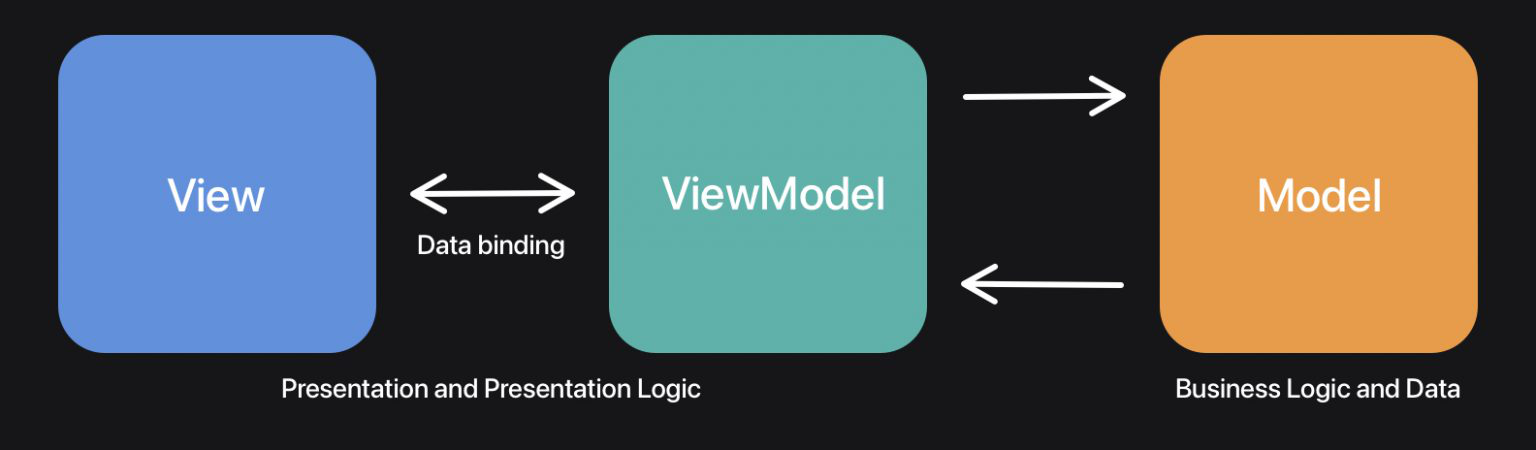
\includegraphics[width=150mm, keepaspectratio]{figures/MVVM-architectural-pattern.png}
    \caption{MVVM minta. \cite{MVVMArchitecture}}
    \label{fig:MVVMArchitecture}
\end{figure}

\section{Rendszer felépítései, komponensei}
\label{sec:Komponents}